\newpage
\section{Описание пользовательского интерфейса}

Пользовательский интерфейс инструмента представляет собой главное окно, в котором пользователь может создавать вкладки (как в браузере).
В каждой вкладке может происходить редактирование различных исходных текстов баз знаний представленных с помощью различных языков. 
По сути, каждая вкладка - это некоторый редактор исходных текстов представленных на некотором внешнем языке. К примеру, это может быть 
редактор sc.g-текстов, редактор sc.n-текстов, редактор sc.s-текстов и т. д.
Набор возможных редакторов определяется набором установленных расширений.

В рамках главного окна имеется панель инструментов, меню приложения, а также для удобства навигации в правой части редактора находится миникарта открытого файла и история его изменений. Меню приложения представляет собой некоторый набор команд. 
Команды, которые отображаются в меню делятся на два типа:
\begin{list}{•}{}
	\item команды, которые являются общими для всех вкладок. В частности к ним относятся команды сохранения, загрузки, помощи и т. д.
	\item команды, которые специфичны для активной вкладки. Зависят от типа активной вкладки.
\end{list}

На панель инструментов, как и в пользовательских интерфейсах большинства приложений, вынесены наиболее часто используемые команды:
\begin{list}{•}{}
	\item \textbf{Создать новый файл} (Ctrl + N) - отображает диалог, в котором пользователю предлагается выбрать формат нового файла.
	Для выбранного пользователем формата создается новая вкладка. Список возможных форматов определяется набором установленных расширений:
	
	\begin{figure}[h]
		\begin{center}
			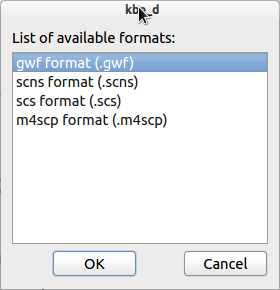
\includegraphics[scale=0.7]{../images/new_dialog.png}
		\end{center}
		\caption{Диалог выбора формата}
		\label{pic_new_dialog}
	\end{figure}
	
	
	\item \textbf{Открыть файл} (Ctrl + O) - открывает диалог выбора файла. Выбранный файл открывается в новой вкладке.
	\item \textbf{Сохранить} (Ctrl + S) - сохраняет содержимое активной вкладки в файл. При этом если содержимое вкладки 
	уже было сохранено в файл или же оно было заргужено из файла, то сохранение будет выполнено именно в этот файл (путь к нему указан в имени вкладки).
	В противном случае поеведение этой команды будет эквивалентно команде \textbf{Сохранить как}
	\item \textbf{Сохранить как} - открывает диалог выбора файла. Содержимое активной вкладки созраняется в выбранный файл.
	\item \textbf{Закрыть} (Ctrl + W) - закртывает активную вкладку. Если в ней имеются не сохраненные даные, то отображается диалог уточняющий необходимость
	их сохранения.
\end{list}

Каким образом выглядит главное окно, можно увидеть на следующем рисунке:
\begin{figure}[h]
	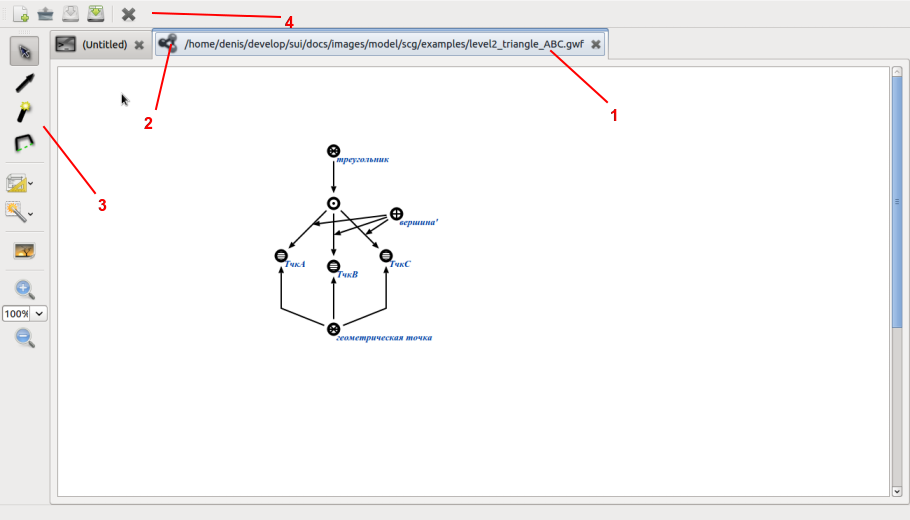
\includegraphics[width=16.23cm, height=9.82cm]{../images/tabs.png}
	\caption{Вкладки в рамках главного окна приложения. 1 - имя вкладки (путь к редактируемому файлу), 2 - иконка, которая показывает
	тип редактируемого текста внутри вкладки, 3 - панель инструментов, расширения в активной вкладке, 4 - основная панель инструментов главного окна, 5 - история изменений текущего файла, 6 - миникарта для быстрой навигации по файлу}
	\label{pic_tabs}
\end{figure}
